%===============================================================================
% zentrale Layout-Angaben und Befehle
%===============================================================================
%
\RequirePackage{ifpdf}
\ifpdf
\documentclass[pdftex, a4paper, 12pt]{article}
\else
\documentclass[a4paper, 12pt]{article}
\fi
\usepackage[utf8]{inputenc}
\usepackage{fancyhdr}
\usepackage[T1]{fontenc}
\usepackage{ae}
\usepackage{color}
\usepackage[printonlyused]{acronym}
%
\ifpdf
\usepackage[pdftex,bookmarksopen,bookmarksnumbered]{hyperref}
\usepackage[pdftex]{graphicx}
\pdfcompresslevel=9
\else
\usepackage{url}
\usepackage[dvips]{graphicx}
\fi
%
% ausführlichere Fehlermeldungen
\errorcontextlines=999
%
% Page-Layout
\setlength\headheight{14pt}
\setlength\topmargin{-15,4mm}
\setlength\oddsidemargin{-0,4mm}
\setlength\evensidemargin{-0,4mm}
\setlength\textwidth{160mm}
\setlength\textheight{252mm}
%
% Absatzeinstellungen
\setlength\parindent{0mm}
\setlength\parskip{2ex}
%
% Anweisung zur Erstellung der Titelseite
% #1 = Name des Seminars
% #2 = Name der Ausarbeitung
% #3 = Autor
% #4 = Betreuer
% #5 = Semester, z.B. SoSe 2002
% #6 = {Bachelor|Master|Diplom}
\renewcommand{\maketitle}[6] {
\pagenumbering{Alph}
  \begin{titlepage}
  \centering
    \begin{minipage}[t]{16cm}
      \begin{minipage}{3cm}
        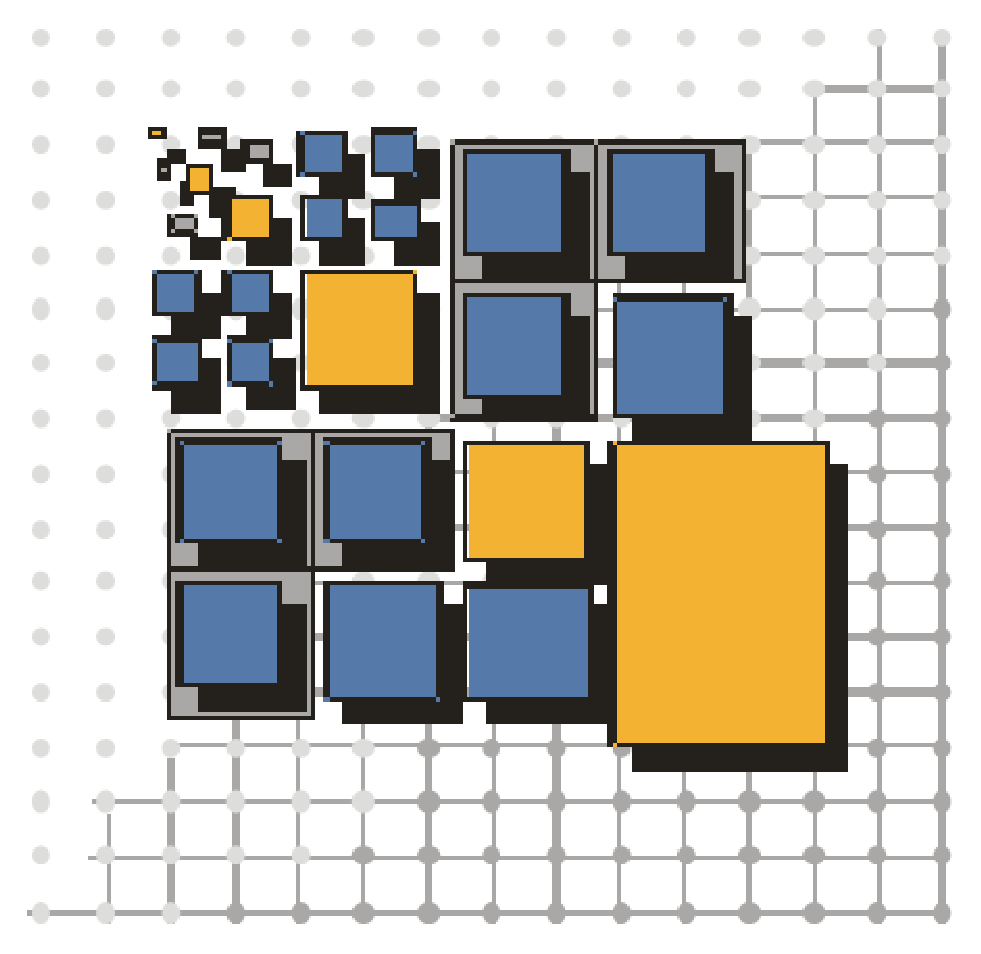
\includegraphics[height=26mm]{include/logo}
      \end{minipage}
      \hfill
      \begin{minipage}{9cm}
        \centering
        Otto-Friedrich-Universität Bamberg\\[12pt]
        {\Large Lehrstuhl für Praktische Informatik}
      \end{minipage}
      \hfill
      \begin{minipage}{3cm}
        
\includegraphics[height=26mm]{include/UB-Logo-neu_blau-cmyk}
      \end{minipage}
    \end{minipage}\\[108pt]
    {\LARGE Ausarbeitung}\\[18pt]
    Im Rahmen des #6-Seminars\\[12pt]
    {\Large\bf #1}\\[92pt]
    Zum Thema:\\[24pt]
    {\Huge #2}\\
    \vfill
    \begin{minipage}{\textwidth}
      \center
      Vorgelegt von:\\
      {\Large #3\\[18pt]}
      Betreuer: #4\\[12pt]
      Bamberg, #5
    \end{minipage}
  \end{titlepage}
}
%
% setzen nur von fusszeile
\newcommand{\setbottom}
{
\pagestyle{fancy}
\fancyhf{}
\fancyfoot[LO]{\footnotesize\sc Lehrstuhl für Praktische Informatik}
\fancyfoot[RO]{\thepage}
\renewcommand{\headrulewidth}{0pt}
\renewcommand{\footrulewidth}{0pt}
}
%
% Einbindung eines Bildes
% #1 = label für \ref-Verweise
% #2 = Name des Bildes ohne Endung relativ zu images-Verzeichnis
% #3 = Beschriftung
% #4 = Breite des Bildes im Dokument in cm
\newcommand{\bild}[4]{%
  \begin{figure}[htb]%
    \begin{center}%
      \includegraphics[width=#4cm]{images/#2}%
      \vskip -0.3cm%
      \caption{#3}%
      \vskip -0,2cm%
      \label{#1}%
    \end{center}%
  \end{figure}%
}
%
% Umgebung für Fliesstext um Grafik
% #1 = Ausrichtung: r, l, i, ...
% #2 = Breite des Bildes in cm
% #3 = Name des Bildes ohne Endung relativ zu images-Verzeichnis
% #4 = Beschriftung
% #5 = label für \ref-Verweise
\newcommand{\fliesstext}[5]{%
\begin{wrapfigure}{#1}{#2cm}%
\includegraphics[width=#2cm]{images/#3}%
\caption{#4}%
\label{#5}%
\end{wrapfigure}%
}
%

\usepackage{listings}
%
% Backgroundcolor
\definecolor{hellgrau}{gray}{0.9}
%
% Configuration
%
\lstdefinestyle{javaStyle}{%
  basicstyle=\small,%
  backgroundcolor=\color{hellgrau},%
  keywordstyle=\bfseries,%
  showstringspaces=false,%
  language=Java,%
  numbers=left,%
  numberstyle=\tiny,%
  stepnumber=1,%
  numbersep=5pt,%
  extendedchars=true,%
  xleftmargin=2em,%
  xrightmargin=2em,%
  lineskip=-1pt,%
  breaklines%
}
%
% Java-Sourcecode environment
% #1 = Caption
% #2 = Label
%
\lstnewenvironment{javacode}[2]%
{\lstset{style=javaStyle,caption=#1,label=#2}}
{}
% Include code from Java-file
% #1 = Filename relative to section-folder
% #2 = Caption
% #3 = Label
%
\newcommand{\javafile}[3]{%
   \lstinputlisting[%
     caption={#2},%
     label={#3},%
     style=javaStyle]{src/#1}%
}

%
\begin{document}
%
% Titelblatt erstellen
\maketitle{Thema des Seminars}{Thema Alles LaTeX Oder Was ?}%
{Autor}{Prof. Dr. Guido Wirtz}{Wintersemester 2013}{Bachelor|Master}
%
% Erstellung der Inhaltsverzeichnisse
\pagenumbering{Roman}
\tableofcontents
\newpage
\listoffigures
\newpage
\listoftables
\newpage
\lstlistoflistings
\newpage
%
% Abkürzungen
%
\section*{Abkürzungsverzeichnis}
% In Klammern steht das längste Akronym!
\begin{acronym}[LSPI]
 \acro{DSG}{Distributed Systems Group}
 \acro{LSPI}{Lehrstuhl für Praktische Informatik}
\end{acronym}
\newpage
\setcounter{page}{1}
\pagenumbering{arabic}
%
% Hier einzelne Kapitel mit \input{Kapitel-File} einf�gen
%
%
\section{Einleitung}
%
Zur Verfassung von Seminar-, Bachelor- und Masterarbeiten bietet die Distributed Systems Group
neben den Word-Vorlagen auch Vorlagen f�r Latex. In diesem Dokument soll
kurz gezeigt, wie die einzelnen Umgebungen und Befehle der Vorlage sinnvoll zur Erstellung
von Arbeiten genutzt werden k�nnen. Es erfolgt aber keine allgemeine Anleitung zur
Erstellung von Dokumenten mit \LaTeX. Als Einstiegsliteratur, die aber f�r die allgemeine
Arbeit mit \LaTeX~durchaus ausreichend ist, eignet sich das Buch von Kopka \cite{kop02}. Eines
der �lteren Werke des Autors reicht ebenfalls aus. 
Eine sehr gute �bersicht �ber alle wichtigen Szenarien gibt das Wikibook "`\LaTeX"' \cite{lat12}.
Weitere hilfreiche Lekt�re findet sich
unter \cite{jue00}, \cite{kue11}, \cite{jue95}, \cite{erb09} und allen verf�gbaren Suchmaschinen.

Die Erstellung eines \LaTeX-Dokumentes erfolgt z.B. �ber die Anweisung \texttt{pdflatex seminar} oder mit einer 
entsprechenden IDE, wie \textit{TeXnicCenter}\footnote{\url{http://www.texniccenter.org}} oder \textit{TeXlipse}\footnote{\url{http://texlipse.sourceforge.net}}.
Hier empfiehlt sich auch das Zusammenspiel mit SumatraPDF\footnote{\url{http://blog.kowalczyk.info/software/sumatrapdf/free-pdf-reader-de.html}}, das eine Vorw�rts- und R�ckw�rtssuche in den Dokumenten erm�glicht. 
%
%
\section{Genereller Aufbau}
%
Die zentrale Datei der Vorlage ist die Datei \texttt{seminar.tex}, die vom Autor f�r jeweilige Arbeit
anzupassen ist. In dieser Datei k�nnen die Einstellungen f�r die Titelseite vorgenommen
werden. Des Weiteren m�ssen in dieser Datei die einzelnen Kapitel der Arbeit, sowie die
\textit{.bib}-Datei mit den \textit{bibtex}-Eintr�gen eingebunden werden.
%
\subsection{Erstellung einer Titelseite}
%
Die Erstellung der Titelseite erfolgt �ber den Befehl \texttt{\textbackslash maketitle}. Die Anzahl der Parameter,
mit der dieser Befehl aufgerufen wird, h�ngt davon ab, ob eine Seminararbeit oder
eine Bachelor-/Masterarbeit erstellt werden soll.
Zur Erstellung einer Titelseite f�r eine Seminararbeit muss der Befehl \texttt{\textbackslash maketitle} mit
sechs Parametern aufgerufen werden.
%
\begin{verbatim}
\maketitle{Thema des Seminars}{Thema der Ausarbeitung}%
{Autor}{Betreuer}{Semester}{Bachelor|Master}
\end{verbatim}
%
Die einzelnen Paramter sind selbsterkl�rend. Falls die Seminararbeit von mehreren Autoren
verfasst wird, sind diese durch \texttt{,\textbackslash\textbackslash} zu trennen. Bei drei Autoren ist also z.B. die
Zeichenkette \texttt{Hans Meier,\textbackslash\textbackslash\ Peter M�ller und\textbackslash\textbackslash\ Hans M�ller} als dritten Parameter
einzusetzen. Als Semesterangabe sollte ein K�rzel wie \texttt{SoSe13} �bergeben werden.

Um die Titelseite einer Abschlussarbeit zu erstellen, ist der Befehl \texttt{\textbackslash maketitle} mit drei
Parametern aufzurufen.
%
\begin{verbatim}
\maketitle{Bachelor-/Masterarbeit}{Studiengang}{Thema der Arbeit}%
{Autor}{Abgabedatum}
\end{verbatim}
%
Auch in diesem Fall sind die Parameter selbsterkl�rend.
%
\subsection{Einbindung der einzelnen Kapitel}
%
Um die �bersichtlichkeit der erstellten Arbeit zu gew�hrleisten, ist es sinnvoll, f�r jedes
Kapitel eine einzelne \textit{.tex}-Datei zu erstellen. 
Damit unter Verwendung dieser Dateien ein einzelnes Dokument erstellt wird, sind die einzelnen Kapitel in der Datei \texttt{seminar.tex}
einzubinden. Dies erfolgt �ber den Befehl \texttt{\textbackslash input}. Soll z.B. ein Kapitel eingef�gt werden,
dass in der Datei \texttt{kapitel-1.tex} enthalten ist, so geschieht dies durch die folgende
Anweisung.

\texttt{\textbackslash input\{kapitel-1\}}

Diese Anweisung ist an der in der Datei \texttt{seminar.tex} markierten Stelle einzuf�gen. 
%
\subsection{Einbindung des Literaturverzeichnisses}
%
Die einzelnen Literaturquellen sind in einer \textit{.bib}--Datei aufzuf�hren. Die \textit{bibtex}--Datei \texttt{example.bib} enth�lt einige Beispiele, wie
verschiedenen Quellen wie Buch, Artikel usw. in dieser Datei aufzuf�hren sind. Jeder der
Eintr�ge ben�tigt zur Referenzierung ein eindeutiges Label, das sich aus den ersten drei
Buchstaben des Nachnamen des Autors und den letzten beiden Ziffern der Jahreszahl der
Ver�ffentlichung ergeben. Sind mehrere Autoren bei einer Literaturquelle aufgef�hrt, so
ergibt sich der Label aus den Anfangsbuchstaben der Nachnamen der ersten drei Autoren
und den letzten beiden Ziffern der Jahreszahl der Ver�ffentlichung. Falls ein Autor in einem
Jahr mehrere Werke ver�ffentlich hat, so sind die weiteren Label mit kleinen Buchstaben,
beginnend bei \textit{b}, zu erg�nzen.

Eine \textit{.bib}-Datei ist mit Hilfe der Anweisung \texttt{\textbackslash bibliography} in der Datei \texttt{seminar.tex} einzubinden.
Die hier verwendete Datei \texttt{references.bib} wurde also durch durch folgende Anweisung
in dieses Dokument eingebunden.

\texttt{\textbackslash bibliography\{references\}}
%
%
\section{Einbindung von Grafiken}
%
Im Allgemeinen werden Grafiken zwischen Absätzen eingefügt. Eine andere
Möglichkeit ist es, die Grafiken von Text umfließen zu lassen. Generell gilt
aber, dass die Grafiken als \emph{pdf}- oder \emph{eps}-Dateien vorliegen
sollten. Dies hängt davon ab, ob \emph{latex} oder \emph{pdflatex} zur Erzeugung
des Dokumentes verwendet wird. Wird \emph{latex} zur Erzeugung genutzt, so
können nur \emph{eps}-Dateien eingebunden werden. Wird das Dokument mit
\emph{pdflatex} erstellt, so sind \emph{pdf}-Dateien zu verwenden.

Grafiken müssen generell im \emph{images}-Verzeichnis vorhanden sein, um sie
erfolgreich einbinden zu können. Selbst erstellte Grafiken müssen also in das
\emph{images}-Verzeichnis kopiert werden.

\subsection{Grafiken zwischen Absätzen}
%
Eine Einbindung von Grafiken zwischen Absätzen erfolgt mit dem Befehl
\texttt{\textbackslash bild}.
\begin{verbatim}
\bild{bild1}{vs-logo}{DSG-Logo}{5}
\end{verbatim}
Der erste Parameter \texttt{bild1} dient als Label für Referenzen auf die
Grafik. Der zweite Parameter ist der Name der Grafikdatei ohne Endung. Als
dritten Parameter ist dem Befehl \texttt{\textbackslash bild} die Beschriftung
der Abbildung zu übergeben. Der letzte Parameter gibt
die Breite der Grafik in cm an. Die Größenangabe darf aber nur als Zahl erfolgen.
Ist eine Grafik breiter als der übergebene Parameter, so wird sie verkleinert, kleinere Grafiken werden
entsprechend vergrößert. Der obige Befehl führt zu der folgenden Abbildung
\ref{bild1}.

\bild{bild1}{vs-logo}{DSG-Logo}{5}

\subsection{Von Text umflossene Grafiken}
%
Sollen Grafiken von Text umflossen werden, so ist der Befehl
\texttt{\textbackslash fliesstext} zu benutzen. Dieser Befehl basiert auf dem Paket
\emph{wrapfig}, dass u.U. nachinstalliert werden muss. Dieses
\fliesstext{r}{3}{vs-logo}{DSG-Logo}{bild2}
Paket ist, wie alle anderen Umgebungen mit dieser Funktionalität, etwas
beschränkt und zum Teil fehlerhaft, deshalb ist die Nutzung nur unter Vorbehalt
empfohlen. Eine Grafik kann wie folgt eingebunden werden.\\\\
\verb+\fliesstext{r}{3}{vs-logo}{DSG-Logo}{bild2}+\\\\
Nach diesem Befehl folgt der Text, der das eingebundene Bild umfliessen
soll. Für den ersten Parameter kommen als einzig relevante Möglichkeiten die
kleinen Buchstaben \emph{l} und \emph{r} in Frage. Diese sorgen für eine
Anordnung der Grafik auf der linken, bzw. rechten Seite. Mit Hilfe des zweiten
Parameters wird die gewünschte Breite der Grafik in cm angegeben, die
entsprechend skaliert wird. Der dritte Parameter ist der Name der Grafikdatei
ohne Endung. Der vierte Parameter bestimmt die Bezeichnung der Grafik. Durch den
fünften Parameter kann ein Label zur Referenzierung angegeben werden.

Eine Eigenheit dieses Pakets ist es, dass Grafiken immer am Anfang eines
Absatzes eingefügt werden. Soll eine Grafik von einem Absatz komplett
umschlossen werden, wie dies bei der Abbildung \ref{bild2} der Fall ist, so ist
der \texttt{\textbackslash fliesstext}-Befehl nicht vor dem Absatz aufzuführen, sondern in
den Text zu integrieren. Der obige \texttt{\textbackslash fliesstext}-Befehl ist demnach
hinter dem Wort "`Dieses"' in den Quelltext eingefügt worden.
%
%
%
\section{Einbindung von Java-Quellcode}
%
Zur Einbindung von Java-Quellcode ist das Paket \emph{listings} notwendig, dass
u.U. nachinstalliert werden muss. Dieses Paket erm�glicht es, dass Quellcode von
verschiedenen Sprachen auf eine �bersichtliche Weise in das Dokument eingebunden
werden kann. Die Einbindung von Java-Quellcode kann auf zwei Arten erfolgen: zum
einen kann der Java-Quellcode im Quelltext des Dokumentes aufgelistet werden,
zum anderen kann der Quellcode aus einer Datei eingelesen werden.

Die Einbindung von Quellcode, der im Quelltext aufgef�hrt ist, muss �ber die
Nutzung einer Umgebung geschehen. Dies soll an einem kleinen Beispiel gezeigt
werden.
\begin{verbatim}
\begin{javacode}{Das ist das erste Listing}{listing1}
public class Test{

  public Test(){
    // mach was
  }

}
\end{javacode}
\end{verbatim}
%
Zun�chst wird eine Umgebung mit der Bezeichnung \texttt{javacode}
erstellt. Als Parameter wird die �berschrift, sowie das Label �bergeben. 
In der Umgebung wird der Java-Quellcode in den Quelltext des Dokumentes eingef�gt und anschlie�end
die Umgebung wieder beendet. Der obige Code erzeugt das folgende Listing
\ref{listing1}.

\begin{javacode}{Das ist das erste Listing}{listing1}
public class Test {

  public Test(){
    // mach was
  }

}
\end{javacode}

Alternativ kann Quellcode auch aus einer Datei eingebunden werden. Dies ist
vorteilhaft, weil die �bersichtlichkeit des Quelltextes verbessert wird. Die
Einbindung einer Quellcode-Datei erfolgt �ber den Befehl
\texttt{\textbackslash javacode}. Damit die Datei erfolgreich eingebunden werden kann, muss
sie im Verzeichnis \texttt{src} liegen. Der Befehl kann wie folgt genutzt werden.
\begin{verbatim}
\javafile{src.java}{Das ist das zweite Listing}{listing2}
\end{verbatim}

Als ersten Parameter muss der Name der Datei (mit Endung) im
\emph{src}-Verzeichnis �bergeben werden. Der zweite Parameter bestimmt die
�berschrift des Listings. Der dritte Parameter dient zur Referenzierung. Es wird
der gleiche Quelltext erstellt, wie in Listing \ref{listing2} zu sehen ist.

\javafile{src.java}{Das ist das zweite Listing}{listing2}
%
%
\section{Nutzung des Abk�rzungsverzeichnisses}
%
Zur Einbindung des Abk�rzungsverzeichnisses wird das \texttt{acronym}--Package\footnote{\url{http://www.ctan.org/tex-archive/macros/latex/contrib/acronym}} verwendet.
Der Eintrag aller verwendeten Abk�rzungen erfolgt in der Datei \texttt{abbreviations.tex}, die bspw. den folgenden Inhalt hat:
%
\begin{verbatim}
	\begin{acronym}[LSPI]
	 \acro{DSG}{Distributed Systems Group}
	 \acro{LSPI}{Lehrstuhl f�r Praktische Informatik}
	\end{acronym}
\end{verbatim}
%
Die geklammerte Abk�rzung \texttt{[LSPI]} sollte dabei durch die l�ngste vorhandene Abk�rzung ersetzt werden.
Eine Abk�rzung wird mit dem Befehl \texttt{\textbackslash acro} innerhalb der \texttt{acronym}--Umgebung definiert.
Standardm��ig werden nur die im Text tats�chlich verwendeten Abk�rzungen auch im Verzeichnis ausgegeben.
Um eine Abk�rzung innerhalb eines Textes einzuf�gen gen�gt der folgende Ausdruck:

\texttt{\textbackslash ac\{}\textit{<acronym>}\texttt{\}}

Bei der ersten Verwendung innerhalb des Textes bewirkt die Anweisung, dass der vollst�ndige Name gefolgt von der Abk�rzung in Klammern ausgegeben wird.
Bei jeder weiteren Verwendung wird lediglich die Kurzform ausgegeben. Die Anweisung \texttt{\textbackslash ac\{DSG\}} erzeugt also zun�chst die Langform "`\ac{DSG}"'.
Anschlie�end nur noch die Abk�rzung "`\ac{DSG}"'.
\newpage
%
% Einstellungen f�r Literaturverzeichnis
\addcontentsline{toc}{section}{\bibname}
\bibliographystyle{IEEEtran}
%
% Hier den bib-file einbinden
\bibliography{bibliography/references}
\end{document}
